\documentclass[letterpaper]{article}
\usepackage[utf8]{inputenc}
\usepackage[margin=1in]{geometry}
\usepackage{parskip, amsmath, hyperref, graphicx, cite}

\title{Atlas: Interactive Visualization of Optimization Loss Surfaces}

\author{
    Sammy Cherna\\\texttt{cherna@mit.edu} \and
    Josh Gruenstein\\\texttt{jgru@mit.edu} \and
    Lior Hirschfeld\\\texttt{liorh@mit.edu} \and
    Martin Schneider\\\texttt{martinfs@mit.edu}
}

\date{18.065 Spring 2019}

\begin{document}

\maketitle

This project largely speaks for itself, so we suggest first checking it out online.  This paper goes into greater depth about how Atlas works, how we built it, and some interesting things you can learn from it. Make sure to watch our intro video as well!

\begin{center}
  \url{https://atls.ml/}
\end{center}

\section{Introduction}
Neural networks have revolutionized image classification, audio processing, and data analysis but largely remain black boxes. Many developers use these models while failing to fully understand the training process, choosing architecture, hyperparameters, and optimizers via grid searches or entirely at random. Recently, visualization techniques have been developed to better understand how these choices impact the training process.

To this end, we have developed \textit{Atlas}, a web application which allows users to plot the loss surface of arbitrary high dimensional functions. This project was largely inspired by ``Visualizing the Loss Landscape of Neural Nets'' by Goldstein et al., which visualizes the loss surface of linear combinations of randomly chosen direction vectors in the network parameter space \cite{li2018visualizing}. As this paper provides only a few static examples, we felt an intuitive, live visualization tool like \textit{Atlas} could help newcomers better understand common questions in optimization, such as:

\begin{list}{}{}
    \item ``Why does this learning rate not work?''
    \item ``Why does changing my activation from ReLu to Sigmoid make training worse?''
    \item ``What does adding more layers actually do to feed-forward neural networks?''
    \item ``What optimization problems are convex, and what aren't?''
    \item ``What do fancy optimizers like Adam and Momentum actually do?''
\end{list}

Our tool answers those questions, not just for toy single variable problems, but for real models on real data.

\section{How it Works}
\subsection{Input Parsing}

Our computation is done in Javascript using Tensorflow.js, but for ease of use we accept normal math syntax as input.  In order to transform said input to Tensorflow.js objects we use Nearley.js, a toolkit that allows us to define a parsing grammar in Backus–Naur form.  This provides an extensible backbone upon which we define both inline operations (such as \texttt{+}) and more complex features such as parenthesizing, matrix transposes, and machine learning functions such as \texttt{softmax} and \texttt{onehot}. 

\subsection{Loss Surface Generation}
Our loss surface visualizes how ``bumpy" a two-dimensional subspace of our weight-space is.  Our ``weight-space" is a concatenation of all the weights of all of our model into a single vector; we  take all of our model's weights, flatten them, and concatenate them into a single large vector. For example, if we had a weight matrix of size [3 x 4] and a bias vector of size [4], we would end up with a weight vector of size [w = 16 3 x 4 + 4 = 16]. We can now consider a two dimensional subspace of our weight space by considering two vectors in this $w$ dimensional space. We'll start by using two randomly generated length $w$ vectors for our axes and will later describe a more refined technique that uses PCA to find basis vectors that empirically produce more useful visualizations.

Computing a loss surface requires a model, data to evaluate the model on, and two basis weight vectors:
\begin{enumerate}
    \item First, we take the (presumably trained) model's current weights and designate then as the center of our plot. If the model has been trained for sufficiently long, the center of our plot should thus represent a local minimum.
    \item We then generate two random weight vectors, where each weight matrix is scaled such that all variables share the same L2 norm.
    \item We then explore the 2D subspace around our central weight vector $w_c$. At each location $(a, b)$ we:
    \begin{enumerate}
        \item Compute the weight vector $w_{ab} = w_c + a * w_a + b * w_b$
        \item Set our model's weights to $w_{ab}$ (by remapping our weight vector back to our weight matrices). 
        \item Evaluate the model's loss on our data.
    \end{enumerate}
    \item Plot the evaluated loss functions at each $(a, b)$ position.
\end{enumerate}

In the vanilla version of the algorithm we generate our two basis vectors randomly. We might get unlucky and end up plotting areas of our weight space that we didn't explore at training time. We can compute better basis vectors through Principle Component Analysis.

While training, we need to record the weight vectors of the model at each time-step. After training, we run PCA on the weight vectors and select the two component vectors with the highest weights. We can then run the rest of the algorithm as normal.  This ensures that training trajectories overlaid on the loss plot make intuitive sense.

\subsection{Plotting}
The plots on \textit{Atlas} have two main components: A loss surface which illustrates the function's shape and a path which shows the model's progression through subsequent epochs of gradient descent.

Generating the surface requires a great deal of computation. To construct a surface with $n$ by $n$ resolution, the entire model must be evaluated $n^2$ times. For this reason, our surfaces often have relatively low granularity. Constructing the path is generally less expensive but still involves a significant amount of prepossessing. To begin, the full weights of the network are recorded after each training step. In all likelihood, none of these intersect with our subspace, so we project each of the corresponding weight vectors onto our two axes. These projected positions generally do not land exactly on a vertex of the surface, whose loss functions we've already computed, so we instead plot the loss value for each point on the path by interpolating between those vertices which are closest to it. This also ensures that the path will appear consistent with the surface we plot, even if we fail to record a local peak/valley.

All plots are constructed using \textbf{plotly.js}, a graphing library built on \textbf{d3.js} and \textbf{stack.gl}. In our plots, we made use of gradient color to convey height in the loss surface and time in gradient descent path.

\subsection{User Interface Design}

Atlas is designed to be user friendly. Usability features include nice math typesetting, loading data from CSV files, and the ability to share workspaces by serializing compressed data into links.  The web-app was built using ES6 Javascript with minimal dependencies and is fairly extensible for future additions.

We intentionally chose to accept math syntax as our model specification method, rather than having a more neural-network-focused UI with features such as dataset loading, representation of layers, etc.  This was a conscious decision to make our tool as general as possible.

\section{Examples}

You can see interactive versions of these examples by clicking on the smiley face in the top right of the website and scrolling past the video. 

\subsection{Simple two-scalar bowl with gradient descent}
Here, we see that the loss surface of $x^2 + y^2$ is a simple bowl, as expected. Note that if only two scalar variables exist, our system automatically aligns the variables to the axes for ease of interpretation.

\begin{center}
    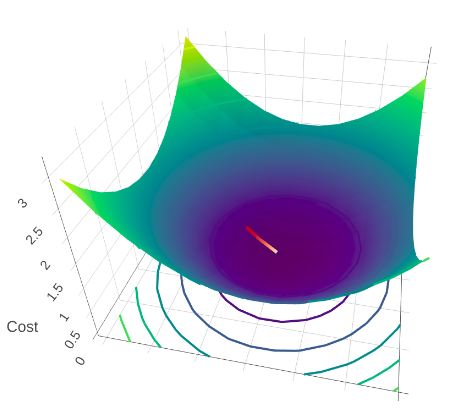
\includegraphics[width=8cm]{simple-bowl.png}
\end{center}

\subsection{Single perceptron softmax classifier on IRIS dataset.}
The IRIS dataset contains 150 records of petal length, sepal length, petal width, sepal, width, and species.  Here, we attempt to predict the species (three options) from the other variables.

Our loss function is: $||A*relu(BX + C) + D - Y||_2$, where $X$ is our data matrix, $Y$ is our target classification matrix, and the other variables are weights. After training for 100 epochs (by which the loss has largely plateaued), we achieve a L2 error of ~6.3.\\

\begin{center}
    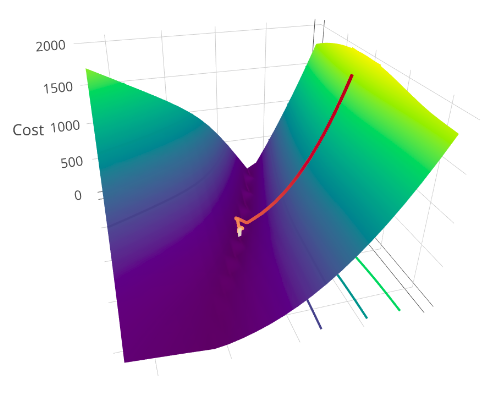
\includegraphics[width=8cm]{single-percepton-iris.png}
\end{center}

\subsection{Three layer Sigmoid network on IRIS dataset.}

We now build a deeper network to try classify species on the IRIS dataset.

Our loss function is $||softmax((A*sigmoid(C*sigmoid(E*X+F)+D)+B)^T)-Y^T||_2$. After training for 2000 epochs, we achieve an L error of ~1.8. This is ~3.5x better than our perceptron classifier. However, as the classifier is more complex, it follows that the loss surface is bumpier and less convex.

\begin{center}
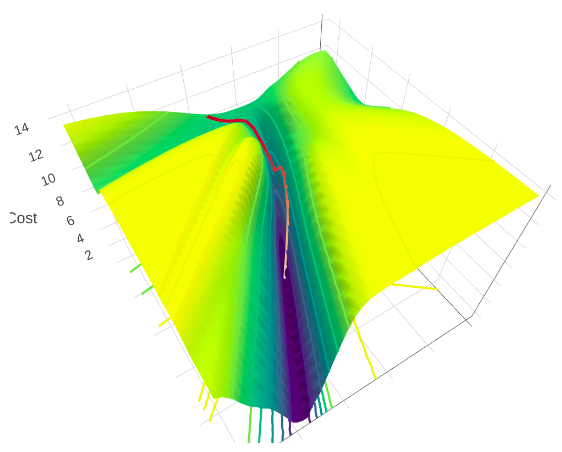
\includegraphics[width=8cm]{three-sigmoid.png}
\end{center}

\subsection{Two layer ReLu network on Boston Housing Prices dataset.}

The Boston Housing Prices dataset contains 506 samples with 14 values each. We predict the price value from the other 13 values. Our loss function is $||A*relu(BX + C) + D - Y||_2$. We observe a smooth training surface, which is unsurprising because we only have two layers. \\

\begin{center}
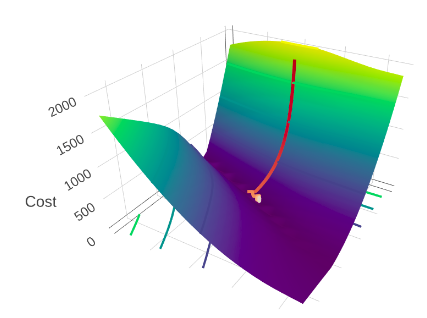
\includegraphics[width=8cm]{two-layer-relu-boston-housing.png}
\end{center}

\section{Discussion}

Throughout experimenting with our tool, we noticed the following issues with our machine learning models (elucidated by the tool):

\begin{itemize}
    \item \textit{Vanishing gradients problem:} When we use ReLU activations in a big network, we often see the loss surface become very flat.  This is a much clearer signal than a flat training curve.
    \item \textit{Too high/low learning rate:} When the learning rate is too high, we see the training bounce around in a rut.  When the learning rate is too low, we see that the surface continues to decrease, so we should run for more epochs.
    \item \textit{Relative bumpiness:} certain activations (such as Softmax and Sigmoid) are very bumpy.  Others are less bumpy.  Bumps are bad, so ReLU is good.
\end{itemize}

The fact that we naturally came across these phenomena is indicative to us that our tool works and is useful for students and practitioners of machine learning.  In the future, we think integrating our tool with something like Ennui (https://math.mit.edu/ennui/) would allow even easier learning and exploration of neural networks.

\bibliography{bibtex}{}
\bibliographystyle{plain}
\end{document}
